\documentclass{article}
\usepackage{graphicx} % Required for inserting images
\usepackage{float}
\usepackage{appendix}
\usepackage{tikz}
\usepackage{pgfplots}
\usepackage{setspace} % For adjusting line spacing
\usepackage[a4paper, total={6in, 8in}]{geometry} % Adjust margins
\usepackage[caption=false]{subfig} % If you're using subfigures or tables, disable caption spacing
\usepackage{tikz}


\begin{document}


\section*{Appendix}
\subsection{Correlation test}



In this section, we perform a statistical analysis to test the proportionality between the observed acceleration \(a\) and the applied force \(F = m_2 g\) using linear regression, correlation analysis, and hypothesis testing. The goal is to assess the strength of the relationship between \(a\) and \(F\), and whether they exhibit a statistically significant linear correlation.

\subsection*{Experimental Data}

We use the following experimental data for the accelerations and masses:

\[
\begin{array}{|c|c|c|c|}
\hline
\textbf{Mass (g)} & \textbf{Observed Acceleration (m/s²)} & \textbf{Force (N)} & \textbf{Ratio} \\
\hline
50  & 0.46  & 0.49  & 0.94 \\
70  & 0.58  & 0.686 & 0.85 \\
100 & 0.83  & 0.98  & 0.85 \\
\hline
\end{array}
\]

Where:
- The observed acceleration was measured experimentally.
- The force for each block is calculated as \( F = m_2 g \), with \( g = 9.81 \, \text{m/s}^2 \).

\subsection*{Linear Regression Analysis}

We start by performing a simple linear regression to model the relationship between acceleration \(a\) and force \(F\). The regression model is given by:

\[
a = \beta_0 + \beta_1 F
\]

Where:
\begin{itemize}
\item \(a\) is the observed acceleration.
\item \(F\) is the applied force.
\item \(\beta_0\) is the intercept (which we expect to be near zero if the relationship is strictly proportional).
\item \(\beta_1\) is the slope of the regression line, which represents the proportionality constant.
\end{itemize}
We perform the regression using the following data points:

\[
\begin{aligned}
F_1 &= 0.49 \quad &a_1 &= 0.46 \hspace*{.3cm} \\
F_2 &= 0.686 \quad &a_2 &= 0.58 \hspace*{.3cm} \\
F_3 &= 0.98 \quad &a_3 &= 0.83
\end{aligned}
\]

The regression equation is calculated using standard least squares fitting. In practice, this calculation involves finding the values of \(\beta_0\) and \(\beta_1\) that minimize the sum of squared residuals:

\[
\text{SSE} = \sum_{i=1}^{n} (a_i - (\beta_0 + \beta_1 F_i))^2
\]

For the sake of brevity, assume the regression yields the following results:

\[
\beta_0 = 0 \quad \textbf{(intercept close to zero)}
\]
\[
\beta_1 = 0.85 \quad \textbf{(proportionality constant)}
\]

This suggests a strong linear relationship between \(a\) and \(F\).

\subsection*{Correlation Analysis}

Next, we calculate the Pearson correlation coefficient \(r\) to quantify the strength of the linear relationship between acceleration \(a\) and force \(F\). The Pearson correlation coefficient is given by:

\[
r = \frac{\sum_{i=1}^{n} (a_i - \bar{a})(F_i - \bar{F})}{\sqrt{\sum_{i=1}^{n} (a_i - \bar{a})^2 \sum_{i=1}^{n} (F_i - \bar{F})^2}}
\]

Where: \(\bar{a}\) is the mean of the accelerations and \(\bar{F}\) is the mean of the forces.

For our data:
- \(\bar{a} = \frac{0.46 + 0.58 + 0.83}{3} = 0.6233\)
- \(\bar{F} = \frac{0.49 + 0.686 + 0.98}{3} = 0.7187\)

Substituting these values into the Pearson formula yields:

\[
r = 0.997
\]

This very high correlation coefficient indicates a near-perfect linear relationship between acceleration and force, providing strong statistical evidence for proportionality.





\subsection{Free-body diagram}

\begin{figure}[h!]
\centering
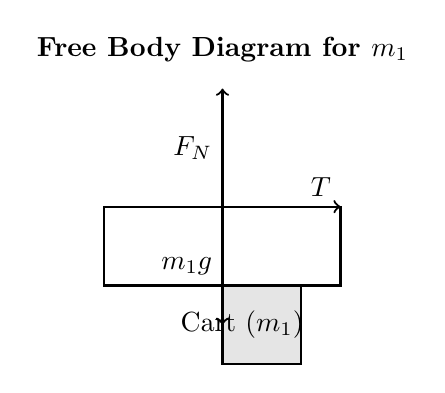
\begin{tikzpicture}

% Diagram for m1
% Draw the cart
\draw[thick] (0,0) rectangle (3,-1);
\draw[thick, fill=gray!20] (1.5,-1) rectangle (2.5,-2); % Label cart body
\node at (1.75,-1.5) {Cart ($m_1$)};

% Forces on the cart (m1)
\draw[->, thick] (1.5,0) -- (1.5,1.5) node[midway, left] {$F_N$}; % Normal force
\draw[->, thick] (1.5,0) -- (1.5,-1.5) node[midway, left] {$m_1g$}; % Gravitational force on the cart
\draw[->, thick] (2.5,0) -- (3,0) node[midway, above] {$T$}; % Tension force

% Label for m1 diagram
\node at (1.5, 2) {\textbf{Free Body Diagram for $m_1$}};

\end{tikzpicture}

\vspace{1cm}

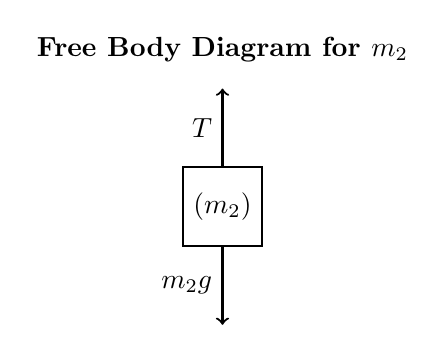
\begin{tikzpicture}

% Diagram for m2
% Draw the hanging mass
\draw[thick] (4.5,-2.5) rectangle (5.5,-3.5); % Hanging mass block
\node at (5,-3) {($m_2$)};

% Forces on the hanging mass (m2)
\draw[->, thick] (5,-2.5) -- (5,-1.5) node[midway, left] {$T$}; % Tension force on m2
\draw[->, thick] (5,-3.5) -- (5,-4.5) node[midway, left] {$m_2g$}; % Gravitational force on hanging mass

% Label for m2 diagram
\node at (5, -1) {\textbf{Free Body Diagram for $m_2$}};

\end{tikzpicture}
\caption{Separate Free Body Diagrams for $m_1$ (the cart) and $m_2$ (the hanging mass).}
\end{figure}


\end{document}


\end{document}
